\documentclass{beamer}
\usepackage[utf8]{inputenc}
\usepackage[french]{babel}

\setbeamertemplate{frametitle}[default][center]

\begin{document} 

	\begin{frame}
	\frametitle{Sommaire}
	\tableofcontents
	\end{frame} 
	
	\section{Général}
	\begin{frame}
	\frametitle{Présentation générale des langages de programmation}
	\begin{itemize}
		\item Les langages de programmation sont en quelque sorte une manière de s'adresser à une machine avec une écriture compréhensible par l'humain
		\pause 
		\item Dans les faits, ils permettent d'écrire des algorithmes mathématiques dans une syntaxe plus ou moins proche de l'algèbre
		\pause 
		\item Ils sont ensuite compilés ou interprétés pour être lus et compris par l'ordinateur
		\pause
		\item Le compilateur/interpréteur transforme le code écrit par le développeur en langage machine (le binaire), compris nativement par la machine		 
	\end{itemize}
	\end{frame}
	
	\subsection{Le niveau d'un langage de programmation}
	\begin{frame}
	\frametitle{Le niveau d'un langage de programmation}
	\begin{itemize}
		\item L'on classe les langages de programmation par "niveaux"
		\pause
		\item Ce niveau représente l'éloignement entre le langage réel de la machine (le binaire) et les constructions qu'on lui superpose.
		\pause
		\item Ainsi, un langage de bas niveau (comme l'assembleur) sera très proche du langage machine et donc bien moins  compréhensible par un humain
		\pause
		\item A contrario, un langage de haut niveau (comme le Java) sera bien mieux compris par l'homme mais comportera de nombreuses couches d'abstraction qui l'éloigneront du langage machine (ce qui peut notamment poser des problèmes d'optimisation sur des dispositifs embarqués et/ou peu puissants)
	\end{itemize}
	\end{frame}
	
		\subsection{Le paradigme d'un langage de programmation}
	\begin{frame}
	\frametitle{Le paradigme d'un langage de programmation}
	\begin{itemize}
		\item Chaque langage de programmation possède un ou plusieurs paradigmes
		\pause
		\item Le paradigme détermine la manière dont le programme va être pensé et rédigé
		\pause
		\item Par exemple, le paradigme impératif décrit une suite d'instructions (d'actions que le programme va exécuter) qui se déroulera de haut en bas, et que rien ne pourra entraver ou modifier
		\pause
		\item D'autres paradigmes existent, tel le paradigme événementiel, où des petites séquences impératives seront exécutées en réaction à des actions prédéfinies; Ou bien l'orienté objet, où l'on déclare des objets qui intéragissent ensemble, etc...
	\end{itemize}
	\end{frame}
	
	\subsection{Différences Compilateur/Interpréteur}
	\begin{frame}
	\frametitle{Différences Compilateur/Interpréteur}
	\begin{itemize}
		\item Un compilateur est un programme qui va transformer le code écrit dans un langage donné (par exemple : le C)  en une séquence d'instructions binaires qui sera exécutée par le processeur.
		\pause
		\item Un interpréteur est un programme qui va lire le code écrit (par exemple : en Python) pour le traduire à la volée en séquences d'instructions binaires compréhensible par la machine.
	\end{itemize}
	\end{frame}	

	\section{C}
	\begin{frame}
	\frametitle{C}
	\begin{columns}

	\begin{column}{3cm}
					
\includegraphics[scale=0.26]{c.png}
	\end{column}

	\begin{column}{7cm}
		\begin{itemize}
			\item Première version : 1972
			\item Auteur : Dennis Ritchie
			\item Paradigmes : Impératif, Procédural, Structuré
			\item Utilisation : Généraliste
			\item Niveau : Haut (Compilé)
			\item Popularité : 2\up{ème} langage le plus utilisé en 2016 (16\%)
		\end{itemize}
	\end{column}
	\end{columns}
	\end{frame}
	
	\section{C++}
	\begin{frame}
	\frametitle{C++}
	\begin{columns}

	\begin{column}{3cm}
				
\includegraphics[scale=0.26]{Langagec++.png}
	\end{column}

	\begin{column}{7cm}
		\begin{itemize}
			\item Première version : 1983
			\item Auteur : Bjarne Stroustrup
			\item Paradigmes : Générique, Objet, Procédural
			\item Utilisation : Généraliste
			\item Niveau : Haut (Compilé)
			\item Popularité : 3\up{ème} langage le plus utilisé en 2016 (7\%)
		\end{itemize}
	\end{column}
	\end{columns}

	\end{frame}
	
	\section{Java}
	\begin{frame}
	\frametitle{Java}
	\begin{columns}

	\begin{column}{3cm}
						
\includegraphics[scale=0.2]{java.png}
	\end{column}

	\begin{column}{7cm}
		\begin{itemize}
			\item Première version : 23 mai 1995
			\item Auteur : Sun MicroSystems
			\item Paradigmes : Objet, Structuré, Impératif, Fonctionnel, Réfléxif
			\item Utilisation : Généraliste/Web
			\item Niveau : Très haut (Pré-Compilé : D'abord compilé en ByteCode, puis interprété par la JVM)
			\item Popularité : 1\up{er} langage le plus utilisé en 2016 (21\%)
		\end{itemize}
	\end{column}
	\end{columns}

	\end{frame}	
	
	\section{C\#}
	\begin{frame}
	\frametitle{C\#}
	\begin{columns}

	\begin{column}{3cm}
			
\includegraphics[scale=0.15]{csharp.jpg} 
	\end{column}

	\begin{column}{7cm}
		\begin{itemize}
			\item Première version : 2000
			\item Auteur : Microsoft
			\item Paradigmes : Objet, Structuré, Impératif
			\item Utilisation : Généraliste/Web
			\item Niveau : Haut (Compilé)
			\item Popularité : 4\up{ème} langage le plus utilisé en 2016 (5\%)
		\end{itemize}
	\end{column}
	\end{columns}
	\end{frame}
	
	\section{Python}
	\begin{frame}
	\frametitle{Python}
	\begin{columns}

	\begin{column}{3cm}
			
\includegraphics[scale=0.2]{python-logo-master-v3-TM.png}
	\end{column}

	\begin{column}{7cm}
		\begin{itemize}
			\item Première version : 1990
			\item Auteur : Guido van Rossum
			\item Paradigmes : Objet, Impératif, Fonctionnelle
			\item Utilisation : Généraliste/Web
			\item Niveau : Très haut (Interprété)
			\item Popularité : 5\up{ème} langage le plus utilisé en 2016 (4\%)
		\end{itemize}
	\end{column}
	\end{columns}
	
	\end{frame}
	
	\section{PHP}	
	\begin{frame}
	\frametitle{PHP}
		\begin{columns}

	\begin{column}{3cm}
			
\includegraphics[scale=0.3]{arton129.png}
	\end{column}

	\begin{column}{7cm}
		\begin{itemize}
			\item Première version : 1994
			\item Auteur : Rasmus Lerdorf
			\item Paradigmes : Impératif, Objet, Fonctionnel, Procédural, Réflexif
			\item Utilisation : Web
			\item Niveau : Très haut (Interprété)
			\item Popularité : 6\up{ème} langage le plus utilisé en 2016 (3\%)
		\end{itemize}
	\end{column}
	\end{columns}
	
	\end{frame}
	
	\section{Visual Basic .NET}	
	\begin{frame}
	\frametitle{Visual Basic .NET}
			\begin{columns}

	\begin{column}{3cm}
			
\includegraphics[scale=0.3]{vb_color.jpg}
	\end{column}

	\begin{column}{7cm}
		\begin{itemize}		 	
			\item Première version : 2001
			\item Auteur : Microsoft
			\item Paradigmes : Objet, Structuré, Impératif
			\item Utilisation : Générique
			\item Niveau : Très haut (Pré-Compilé : D'abord compilé en CIL, puis interprété par l'interpréteur .NET)
			\item Popularité : 7\up{ème} langage le plus utilisé en 2016 (3\%)
		\end{itemize}
	\end{column}
	\end{columns}
	
	\end{frame}
	
	\section{JavaScript}
	\begin{frame}
	\frametitle{JavaScript}
	\begin{columns}

	\begin{column}{3cm}
				
\includegraphics[scale=0.3]{javascript_logo.png}
	\end{column}

	\begin{column}{7cm}
		\begin{itemize}
			\item Première version : 1995
			\item Auteur : Brendan Eich
			\item Paradigmes : Script, Objet, Fonctionnel, Impératif
			\item Utilisation : Web
			\item Niveau : Très haut (Interprété)
			\item Popularité : 8\up{ème} langage le plus utilisé en 2016 (3\%)
		\end{itemize}
	\end{column}
	\end{columns}

	\end{frame}

	\section{Assembleur}
	\begin{frame}
	\frametitle{Assembleur}
	\begin{columns}
	\begin{column}{3cm}
				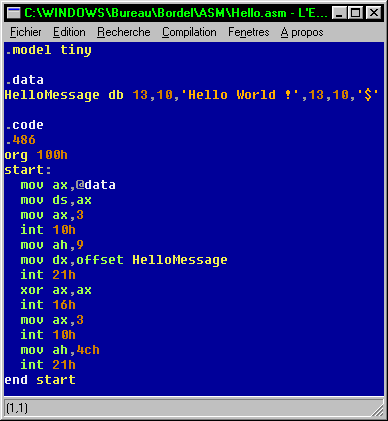
\includegraphics[scale=0.3]{asm.png}
	\end{column}
	\begin{column}{7cm}
		\begin{itemize}
			\item Première version : 1954
			\item Auteur : 	Nathaniel Rochester
			\item Utilisation : Codage bas niveau/Informatique embarquée
			\item Niveau : Bas (Langage Machine)
			\item Popularité : 9\up{ème} langage le plus utilisé en 2016 (2\%)
		\end{itemize}
	\end{column}
	\end{columns}
	\end{frame}
	
\end{document}